\documentclass[a4paper]{article}
\usepackage[utf8]{inputenc}
\usepackage[spanish, es-tabla]{babel}

\usepackage{amsmath}
\usepackage{amsfonts}
\usepackage{amssymb}

\usepackage{float}
\usepackage{graphicx}
\usepackage{subcaption}
\captionsetup{compatibility=false}

\usepackage{multirow}
\setlength{\doublerulesep}{\arrayrulewidth}

\usepackage{array}
\newcolumntype{C}[1]{>{\centering\let\newline\\\arraybackslash\hspace{0pt}}m{#1}}

\usepackage[american]{circuitikz}

\usepackage{fancyhdr}

\usepackage{units} 
\pagestyle{fancy}
\fancyhf{}
\lhead{22.11 Electrónica I}
\rhead{Mechoulam, Lambertucci, Rodriguez, Londero}
\rfoot{Página \thepage}



\begin{document}

%%%%%%%%%%%%%%%%%%%%%%%%%%%%%%%%%%%%%%%%%%%%%%%%%%%%%%%%%%%%%%%%%%%%%%%%% 
%								CARATULA								%
%%%%%%%%%%%%%%%%%%%%%%%%%%%%%%%%%%%%%%%%%%%%%%%%%%%%%%%%%%%%%%%%%%%%%%%%% 

\begin{titlepage}
\newcommand{\HRule}{\rule{\linewidth}{0.5mm}}
\center
\mbox{\textsc{\LARGE \bfseries {Instituto Tecnológico de Buenos Aires}}}\\[1.5cm]
\textsc{\Large 22.11 Electrónica I}\\[0.5cm]


\HRule \\[0.6cm]
{ \Huge \bfseries Trabajo práctico N$^{\circ}$1}\\[0.4cm] 
\HRule \\[1.5cm]


{\large

\emph{Grupo 3}\\
\vspace{3px}

\begin{tabular}{lr} 	
\textsc{Mechoulam}, Alan  &  58438\\
\textsc{Lambertucci}, Guido Enrique  & 58009 \\
\textsc{Rodriguez Turco}, Martín Sebastian  & 56629 \\
\textsc{Londero Bonaparte}, Tomás Guillermo  & 58150 \\
\end{tabular}

\vspace{20px}

\emph{Profesores}\\
Alcocer, Fernando\\
Oreglia, Eduardo Victor\\
Gardella, Pablo Jesús\\
\vspace{3px}
%\textsc{} \\	

\vspace{100px}

\begin{tabular}{ll}

Presentado: & 24/09/19\\

\end{tabular}

}

\vfill

\end{titlepage}


%%%%%%%%%%%%%%%%%%%%%%%%%%%%%%%%%%%%%%%%%%%%%%%%%%%%%%%%%%%%%%%%%%%%%%%%% 
%								INFORME									%
%%%%%%%%%%%%%%%%%%%%%%%%%%%%%%%%%%%%%%%%%%%%%%%%%%%%%%%%%%%%%%%%%%%%%%%%%

\section{Introducción}
La configuración a estudiar en este informe será la configuración de \textbf{Bootstrap}. El bootstraping es una técnica usada para aumentar al impedancia de entrada y bajar la impedancia de salida utilizando un capacitor para realimentar el emisor con la base del transistor. El circuito propuesto es un colector común utilizando el capcitor C2 para la realimentación:
\begin{figure} [H]
	\centering
	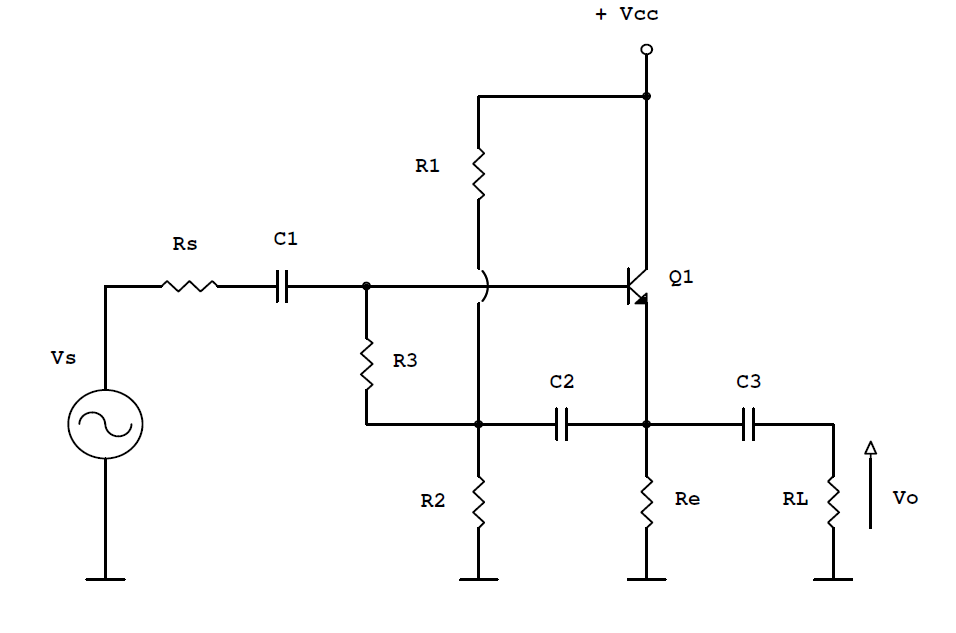
\includegraphics[width=0.6\textwidth]{imagenes/bootstrap.PNG}
	\caption{Circuito Bootstrap propuesto.}
	\label{fig:boot}
\end{figure}

\section{Desarrollo}

\subsection{Polarización}
El primer paso será pasivar la fuente Vs y tratar los capacitores como un circuito abierto. Redibujando y utilizando el teorema de Thevenin se llega a las siguientes condiciones:
\begin{figure} [H]
	\centering
	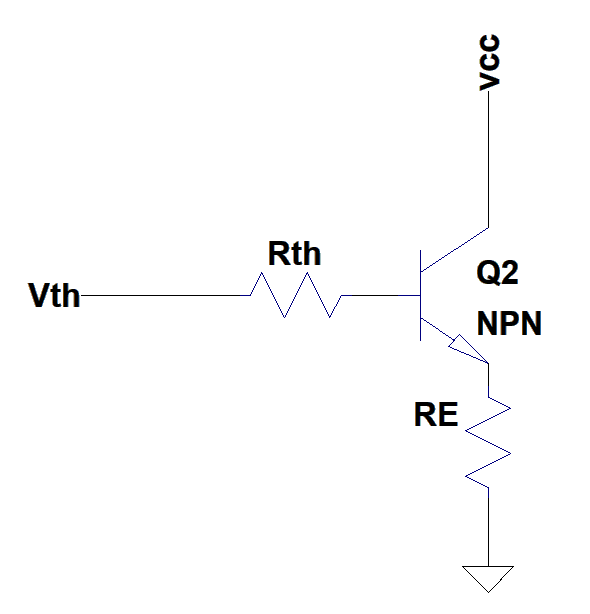
\includegraphics[width=0.5\textwidth]{imagenes/polarizacion.PNG}
	\caption{Circuito Bootstrap Polarización.}
	\label{fig:pol}
\end{figure}
donde:
\begin{align} V_{Th}= V_{cc}\cdot \frac{R_2}{R_1+R_2} \ \ R_{Th}= (R_1 // R_2) +R_3\end{align}
Recorriendo la malla de entrada se obtienen la siguientes ecuaciones:
\begin{align} V_{Th}-I_b \cdot R_{Th} -V_{BE_{On}}-I_e \cdot R_E=0  \ \  I_b\approx  \beta \cdot I_e\end{align}
Obteniendo las siguientes expresiones apra $I_C$ y $V_{ce}$:
\begin{align} I_{C}\approx \frac{V_{Th}-V_{BE_{On}}}{\frac{R_{Th}}{1+\beta}+R_E} \ \ V_{ce}= V_{cc}-I_c\cdot R_E\end{align}
\subsection{Modelo Incremental}
Para el modelo incremental se utilizarán los siguientes estimadores:
\begin{align}\hat{hfe}=\beta \ \ \ \  \hat{hie} = \frac{V_T}{I_b} \ \ \ \ \hat{\frac{1}{hoe}} = \frac{V_a}{I_c}\end{align}
Siendo este el circuito correspondiente al modelo:
\begin{figure} [H]
	\centering
	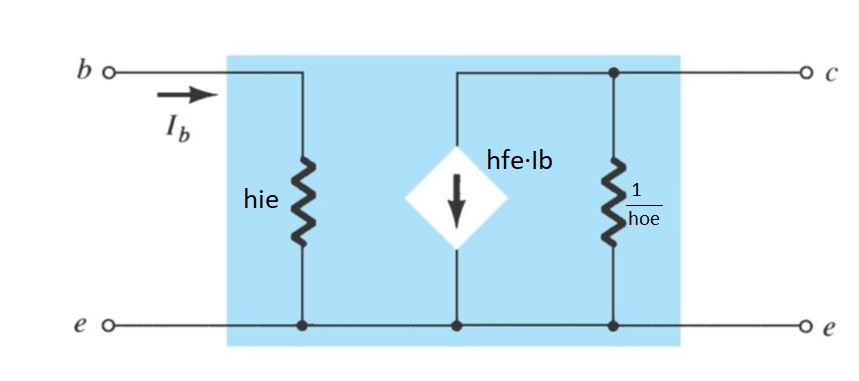
\includegraphics[width=\textwidth]{imagenes/modeloincremetnal.jpg}
	\caption{Modelo incremental.}
	\label{fig:modinc}
\end{figure}
Para nuestro transistor en particular se midió el HFE siendo este $HFE \approx 380 $
\subsection{Circuito Incremental}
Reemplazando el transistor por su modelo incremental, asumiendo que se trabaja con pequeñas señales a frecuencias medias se obtiene el siguiente circuito
\begin{figure} [H]
	\centering
	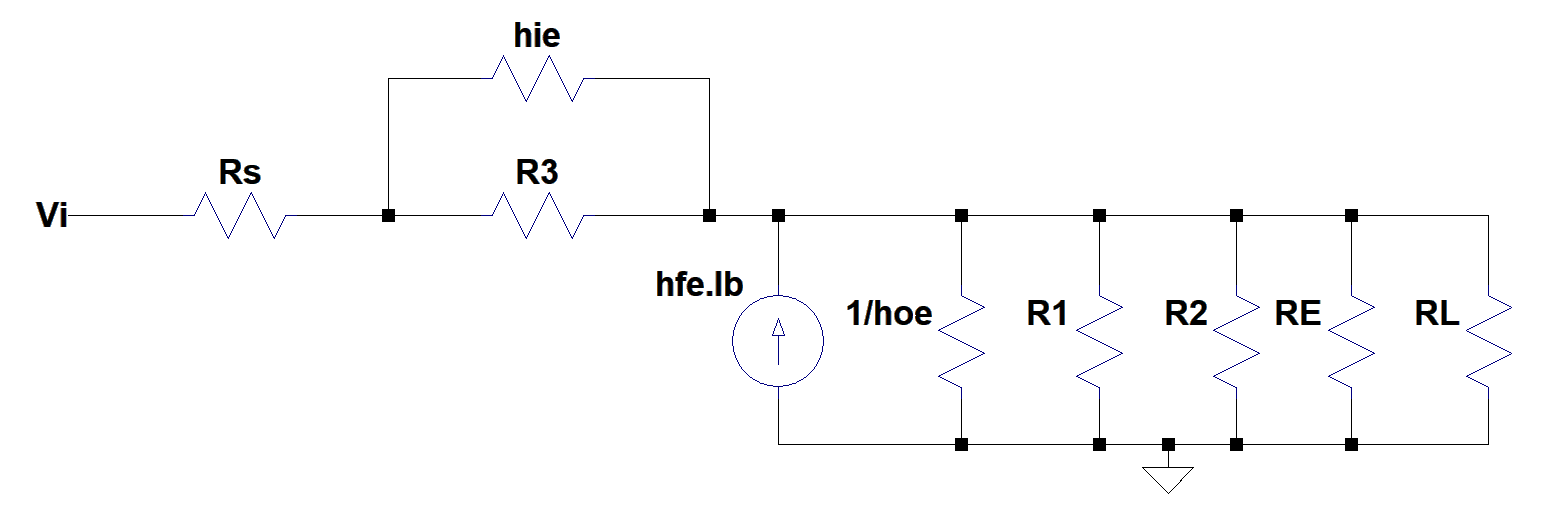
\includegraphics[width=\textwidth]{imagenes/circinc.png}
	\caption{Circuito incremental.}
	\label{fig:circinc}
\end{figure}
Redibujando convenientemente y utilizado el pasaje a nivel de corriente se puede describir el circuito como:

\begin{figure} [H]
	\centering
	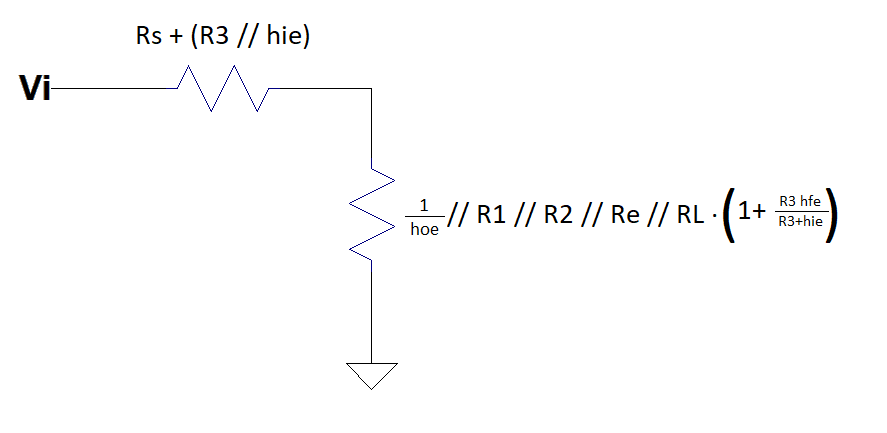
\includegraphics[width=\textwidth]{imagenes/circinc2.png}
	\caption{Circuito incremental final.}
	\label{fig:circinc2}
\end{figure}
Una pequeña modificacion que se hace a la expresión del circuito es definir un hfe efectivo y un hie efectivo, estos siendo para el circuito:
\begin{align} hfe^* = hfe\cdot \frac{r_3}{R_3+hie} \ \ \ \ hie^* = R_3 // hie \end{align}
\subsection{Elección de componentes.}
Se eligió un punto de operación \textbf{Q} tal que la tensión colector-emisor $V_{ce} = 5 V$ y la corriente de colector $I_{cq} = 2mA$, para estos valores se eligió valores de resistencia que cumplan dicho punto de polarización, recorriedo la malla de entrada y salida para elegirlos. Se eligieron:
$R_1 = 10k\Omega \ \ \ R_2 = 14.7 k\Omega \ \ \ R_3 = 1 k\Omega \ \ \ R_E = 2.2k\Omega \ \ \ $
se tomó como resistencia del generador $R_s \approx 50 \Omega$ y $R_L \approx 10k\Omega $ los valores de capacitores elegidos fueron tal que su impedancia sea despreciable frente a las resistencias para valores de frecuencias medias, tomando vcc=10V.
\subsection{Resultados de interés.}
Nos centraremos en la ganancia de Tensión, Corriente, impedancia de entrada y salida:
\begin{equation} \Delta V = \frac{V_o}{V_i} = \frac{ \left(\frac{1}{hoe} // R_1 // R_2 // R_E // R_L  \right)\cdot (1+hfe^*)}{R_s + hie^* + \left(\frac{1}{hoe} // R_1 // R_2 // R_E // R_L  \right)\cdot (1+hfe*) } 
\end{equation}
\begin{equation} \Delta I = \frac{I_o}{I_i} =  \frac{\frac{1}{hoe} // R_1 // R_2 // R_E}{\frac{1}{hoe} // R_1 // R_2 // R_E+R_L} \cdot (1+hfe^*)
\end{equation}
\begin{equation} Z_{In} = R_s + hie^* + \left(\frac{1}{hoe} // R_1 // R_2 // R_E // R_L  \right)\cdot (1+hfe*)\end{equation}
\begin{equation} Z_{Out} = \frac{(R_s + hie^*)}{(1+hfe*)} //  \left(\frac{1}{hoe} // R_1 // R_2 // R_E // R_L  \right)\end{equation}
Luego se graficó la ganancia de tensión en función de la frecuencia:
\begin{figure} [H]
	\centering
	\includegraphics[width=\textwidth]{imagenes/avs.png}
	\caption{Transferencia Módulo.}
	\label{fig:transmod}
\end{figure}
\begin{figure} [H]
	\centering
	\includegraphics[width=\textwidth]{imagenes/avsp.png}
	\caption{Transferencia Fase.}
	\label{fig:transph}
\end{figure}
Se midió la impedancia de entrada para frecuencias medias, las cuales fueron entre 1kHz y 10 kHz, obteniendio un valor de $Z_{in}=83.4k\Omega$ y midiendo la impedancia de salida se obtuvo un valor de $Z_{out} = 9.86 k \Omega $
Dichas mediciones coinciden parcialmente con la simulación, las discrepancias se deben principalmente a los cambios en el HFE, los cuales son esperables, pero dadoa  que la impedancia de entrada es grande y la de salida pequeña se toman como válidos.

\end{document}
